\documentclass[conference]{IEEEtran}
\IEEEoverridecommandlockouts
% The preceding line is only needed to identify funding in the first footnote. If that is unneeded, please comment it out.
%----------------------------------------------------------
\usepackage{cite}
\usepackage[pdftex]{graphicx}
% declare the path(s) where your graphic files are
\graphicspath{images/}
\DeclareGraphicsExtensions{.pdf,.jpeg,.png,.jpg}
\usepackage{amsmath,amssymb,amsfonts}
\usepackage{algorithmic}
\usepackage{graphicx}
\usepackage{textcomp}
\usepackage{array}
%\usepackage[caption=false,font=normalsize,labelfont=sf,textfon =sf]{subfig}
\usepackage{dblfloatfix}
\usepackage{url}
\usepackage{lipsum}
\usepackage{listings}
\usepackage{xcolor}
\def\BibTeX{{\rm B\kern-.05em{\sc i\kern-.025em b}\kern-.08em
    T\kern-.1667em\lower.7ex\hbox{E}\kern-.125emX}}
%----------------------------------------------------------
    \lstset{
        escapeinside={/*@}{@*/},
        language=Python,	
        basicstyle=\fontsize{8.5}{12}\selectfont,
        numbers=left,
        numbersep=2pt,    
        xleftmargin=2pt,
        frame=tb,
        columns=fullflexible,
        showstringspaces=false,
        tabsize=4,
        keepspaces=true,
        showtabs=false,
        showspaces=false,
        morekeywords={inline,public,class,private,protected,struct},
        captionpos=b,
        lineskip=-0.4em,
        aboveskip=10pt,
        extendedchars=true,
        breaklines=true,
        prebreak = \raisebox{0ex}[0ex][0ex]{\ensuremath{\hookleftarrow}},
        keywordstyle=\color[rgb]{0,0,1},
        commentstyle=\color[rgb]{0.133,0.545,0.133},
        stringstyle=\color[rgb]{0.627,0.126,0.941},
    }
%----------------------------------------------------------
\newcommand\largurafig{9cm}
\newcommand\recuodot{0.03cm}

\begin{document}

\title{Jogo Pong\\
{\footnotesize \textsuperscript{*} Sistemas Embarcados: Prof. Marco Reis - marco.reis@ba.docente.senai.brr}
\thanks{Identify applicable funding agency here. If none, delete this.}
}

% \author{\IEEEauthorblockN{Marco Reis, 41650-010\IEEEauthorrefmark{1}}
% \IEEEauthorblockA{\IEEEauthorrefmark{1}Robotics & Autonomous Systems Center,
% Senai Cimatec, Salvador, Brazil}% <-this % stops an unwanted space



\author{\IEEEauthorblockN{1\textsuperscript{st} Alexandre Adonai Gama da Silva}
\IEEEauthorblockA{\textit{IEEE - EMBS} \\
\textit{Senai - CIMATEC}\\
Salvador, Brasil \\
alexandre.s@aln.senaicimatec.edu.br}
\and
\IEEEauthorblockN{2\textsuperscript{nd} João Gabriel da Anunciação Calmon}
\IEEEauthorblockA{\textit{IEEE - RAS} \\
\textit{Senai - CIMATEC}\\
Salvador, Brasil \\
joao.calmon@aln.senaicimatec.edu.br}
\and
\IEEEauthorblockN{3\textsuperscript{rd} João Vitor Silva Mendes}
\IEEEauthorblockA{\textit{Instituto Senai ILMA} \\
\textit{Senai - CIMATEC}\\
Salvador, Brasil \\
joao.mendes@aln.senaicimatec.edu.br}
}

\maketitle

\begin{abstract}
---
\end{abstract}

\begin{IEEEkeywords}
Processing 3, Arduino, Pong, Maker
\end{IEEEkeywords}

\section{Introdução}


\section{Componentes Utilizados}

\subsection{Arduino UNO}


\section{Execução do projeto}

\subsection{---}\label{AA}


\subsection{---}

\subsection{Comunicação Serial}
Para a realização da troca de dados entre o Arduino e o computador, mais especificamente o \emph{processing}, foi utilizado o cabo USB AB do Arduino, o mesmo empregado no processo de inscrição de novos códigos na placa. Quanto ao padrão de envio das informações, a mesma se deu de forma serial, ou seja, um bit é enviado após o outro de forma sequencial \cite{ArduinoHomepage}. Como haviam quatro informações que deveriam ser enviadas a cada ciclo, a saber a leitura analógica dos dois potenciômetros e a leitura digital dos dois \emph{pushbuttons}, foi preciso estabelecer um padrão de envio para que estes dados pudessem ser separados no momento da leitura. 

Para construção de um padrão de formatação das \emph{strings} o caractere '-' foi empregado como separador entre um valor inteiro e o outro, sempre escritos na mesma ordem, e finalizado pelo caractere de quebra de linha. O resultado obtido foram \emph{strings} no seguinte formato: "potenciômetro1 - potenciômetro2 - botão pause - botão reset \textbackslash n", no qual cada nome representa o valor lido em cada um dos componentes.

Em posse dessa configuração foi possível utilizar as funções \emph{readStringUntil()}, responsável por ler as informações da porta serial até o caractere informado como parâmetro ao método) e a \emph{split()}, responsável por separar uma \emph{string} em outras menores com base no parâmetro passado. Vale ressaltar que ambas são funções já implementadas no \emph{processing 3} \cite{ProcessingHomepage}.


\subsection{Sistema de Rebatimento}
Para criação do sistema de rebatimento, o qual deveria retornar a bola com uma angulação diferente a depender da região da barra atingida, foi tomado como base o valor do centro da barra na tela naquele instante (o mesmo valor usado para a sua movimentação) e a sua altura total, ou seja, um valor fixo. A fim de dividir a barra em oito seções de mesmo tamanho, conforme a figura ~\ref{fig:barra_dividida} foi considerado que a divisa entre elas estava a uma distância de um oitavo da altura da barra uma das outras e somando n/8 (com n variando de 1 a 4) ao valor da posição do centro da barra se obteve a divisão da parte superior e aplicando-se o mesmo procedimento, exceto pelo sinal oposto (subtração), foi possível realizar essa mesma operação para a as divisões abaixo do centro da barra.

\begin{figure}[htbp]
\centerline{
    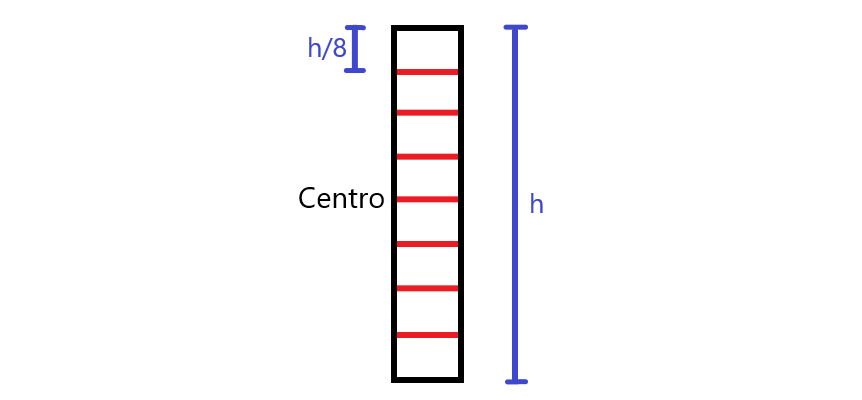
\includegraphics[width = \largurafig]{images/barra_dividida.png}
    }
\caption{Divisão das barras de rebatimento.}
\label{fig:barra_dividida}
\end{figure}

Durante o momento de encontro da bola com a barra, a fim de identificar a região de colisão, foi aplicada uma sequência de estruturas condicionais começando as verificações pelos dois seguimentos centrais, isto é, se a coordenada vertical da bola estava à uma distância menor ou igual a um oitavo do centro da barra, e então partindo gradualmente para aqueles que se encontravam a uma unidade de distância acima ou abaixo do anterior até chegar às extremidades através do aumento do valor da distância (um oitavo, depois dois oitavos, três oitavos e por fim quatro oitavos). É evidente que algumas das frações anteriores poderiam ser simplificadas, contudo, optou-se por manter todas elas com denominador comum 8 para que pudessem ser comparadas mais facilmente e para ressaltar a ideia de que a barra fora dividida em 8 segmentos para construção deste sistema.

Vale ressaltar que a ordem das verificações é importante para a tarefa, já que todos os seguimentos estão contidos numa distância de metade da altura da barra, mas apenas os dois centrais estão contidas numa distância de um oitavo da altura da barra. Ou seja, se a condição mais abrangente fosse verificada primeiro, as mais restritivas jamais seriam alcançadas, já que elas já estariam inclusas na primeira.

O rebatimento em ângulo foi desenvolvido empregando conceitos de trigonometria e algumas operações vetoriais. Ora, sabendo que a velocidade pode ser presentada por um vetor de módulo v num plano bidimensional x e y, é possível traçar um triângulo retângulo de ângulo $\theta$, componentes x, y e hipotenusa igual ao modulo da velocidade, como mostrado na figura ~\ref{fig:modulo}. No momento do rebatimento são conhecidos os valores de velocidade nos eixos x e y (já que foi este o formato adotado para a movimentação da bola), enquanto no instante após a rebatida é conhecido o novo ângulo desejado, informado como parâmetro previamente. Considerando que o rebatimento não acelera nem desacelera a bola (não há perdas, a energia é conservada e nenhuma energia externa é adicionada ao sistema), apenas o seu ângulo é mudado e é possível inferir que o modulo da velocidade antes e após este momento se mantem mesmo. Assim, tal processo pode ser entendido como a rotação de um vetor em relação a um eixo que passa por uma de suas extremidades, de maneira analogo ao que é mostrado na figura ~\ref{fig:rotacao}. Logo, como as coordenadas x e y antes do rebatimento são conhecidas é possível calcular a hipotenusa do triângulo traçado (modulo da velocidade) e em posse de uma informação do ângulo de rebatimento desejado e da hipotenusa já obtida se torna fácil obter as novas velocidades nos eixos x e y por meio das relações de seno e cosseno, que são passadas como parâmetros para a função de movimentação da bola.

\begin{figure}[htbp]
\centerline{
    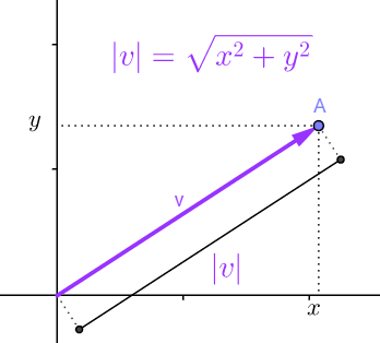
\includegraphics[width = \largurafig]{images/modulo_vetor.jpg}
    }
\caption{Modulo de um vetor.}
\label{fig:modulo}
\end{figure}

\begin{figure}[htbp]
\centerline{
    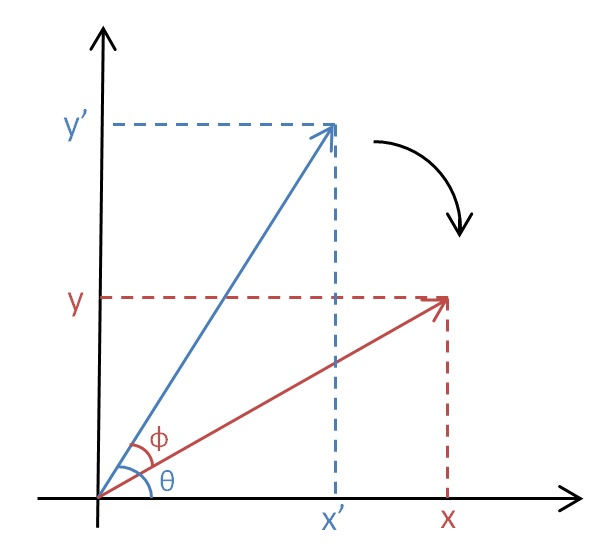
\includegraphics[width = \largurafig]{images/rotação_vetor.png}
    }
\caption{Rotação de um vetor.}
\label{fig:rotacao}
\end{figure}

\subsection{Equations}
\begin{equation}
a+b=\gamma\label{eq}
\end{equation}


\subsection{\LaTeX-Specific Advice}

Please use ``soft'' (e.g., \verb|\eqref{Eq}|) cross references instead
of ``hard'' references (e.g., \verb|(1)|). That will make it possible
to combine sections, add equations, or change the order of figures or
citations without having to go through the file line by line.

Please don't use the \verb|{eqnarray}| equation environment. Use
\verb|{align}| or \verb|{IEEEeqnarray}| instead. The \verb|{eqnarray}|
environment leaves unsightly spaces around relation symbols.

Please note that the \verb|{subequations}| environment in {\LaTeX}
will increment the main equation counter even when there are no
equation numbers displayed. If you forget that, you might write an
article in which the equation numbers skip from (17) to (20), causing
the copy editors to wonder if you've discovered a new method of
counting.

{\BibTeX} does not work by magic. It doesn't get the bibliographic
data from thin air but from .bib files. If you use {\BibTeX} to produce a
bibliography you must send the .bib files. 

{\LaTeX} can't read your mind. If you assign the same label to a
subsubsection and a table, you might find that Table I has been cross
referenced as Table IV-B3. 

{\LaTeX} does not have precognitive abilities. If you put a
\verb|\label| command before the command that updates the counter it's
supposed to be using, the label will pick up the last counter to be
cross referenced instead. In particular, a \verb|\label| command
should not go before the caption of a figure or a table.

Do not use \verb|\nonumber| inside the \verb|{array}| environment. It
will not stop equation numbers inside \verb|{array}| (there won't be
any anyway) and it might stop a wanted equation number in the
surrounding equation.

\subsection{Some Common Mistakes}\label{SCM}
\begin{itemize}
\item The word ``data'' is plural, not singular.
\item The subscript for the permeability of vacuum $\mu_{0}$, and other common scientific constants, is zero with subscript formatting, not a lowercase letter ``o''.
\item In American English, commas, semicolons, periods, question and exclamation marks are located within quotation marks only when a complete thought or name is cited, such as a title or full quotation. When quotation marks are used, instead of a bold or italic typeface, to highlight a word or phrase, punctuation should appear outside of the quotation marks. A parenthetical phrase or statement at the end of a sentence is punctuated outside of the closing parenthesis (like this). (A parenthetical sentence is punctuated within the parentheses.)
\item A graph within a graph is an ``inset'', not an ``insert''. The word alternatively is preferred to the word ``alternately'' (unless you really mean something that alternates).
\item Do not use the word ``essentially'' to mean ``approximately'' or ``effectively''.
\item In your paper title, if the words ``that uses'' can accurately replace the word ``using'', capitalize the ``u''; if not, keep using lower-cased.
\item Be aware of the different meanings of the homophones ``affect'' and ``effect'', ``complement'' and ``compliment'', ``discreet'' and ``discrete'', ``principal'' and ``principle''.
\item Do not confuse ``imply'' and ``infer''.
\item The prefix ``non'' is not a word; it should be joined to the word it modifies, usually without a hyphen.
\item There is no period after the ``et'' in the Latin abbreviation ``et al.''.
\item The abbreviation ``i.e.'' means ``that is'', and the abbreviation ``e.g.'' means ``for example''.
\end{itemize}
An excellent style manual for science writers is \cite{young1989technical}.

\subsection{Authors and Affiliations}
\textbf{The class file is designed for, but not limited to, six authors.} A 
minimum of one author is required for all conference articles. Author names 
should be listed starting from left to right and then moving down to the 
next line. This is the author sequence that will be used in future citations 
and by indexing services. Names should not be listed in columns nor group by 
affiliation. Please keep your affiliations as succinct as possible (for 
example, do not differentiate among departments of the same organization).

\subsection{Identify the Headings}
Headings, or heads, are organizational devices that guide the reader through 
your paper. There are two types: component heads and text heads.

Component heads identify the different components of your paper and are not 
topically subordinate to each other. Examples include Acknowledgments and 
References and, for these, the correct style to use is ``Heading 5''. Use 
``figure caption'' for your Figure captions, and ``table head'' for your 
table title. Run-in heads, such as ``Abstract'', will require you to apply a 
style (in this case, italic) in addition to the style provided by the drop 
down menu to differentiate the head from the text.

Text heads organize the topics on a relational, hierarchical basis. For 
example, the paper title is the primary text head because all subsequent 
material relates and elaborates on this one topic. If there are two or more 
sub-topics, the next level head (uppercase Roman numerals) should be used 
and, conversely, if there are not at least two sub-topics, then no subheads 
should be introduced.

\subsection{Figures and Tables}
\paragraph{Positioning Figures and Tables} Place figures and tables at the top and 
bottom of columns. Avoid placing them in the middle of columns. Large 
figures and tables may span across both columns. Figure captions should be 
below the figures; table heads should appear above the tables. Insert 
figures and tables after they are cited in the text. Use the abbreviation 
``Fig.~\ref{fig}'', even at the beginning of a sentence.


\section*{Acknowledgment}

The preferred spelling of the word ``acknowledgment'' in America is without an ``e'' after the ``g''. Avoid the stilted expression ``one of us (R. B. G.) thanks $\ldots$''. Instead, try ``R. B. G. thanks$\ldots$''. Put sponsor acknowledgments in the unnumbered footnote on the first page.

\section*{References}

Please number citations consecutively within brackets \cite{eason1955certain}.
The sentence punctuation follows the bracket \cite{clerk1892maxwell}. Refer simply to the reference number, as in \cite{jacobs1963fine}---do not use ``Ref. \cite{jacobs1963fine}'' or ``reference \cite{jacobs1963fine}'' except at 
the beginning of a sentence: ``Reference \cite{jacobs1963fine} was the first $\ldots$''

Number footnotes separately in superscripts. Place the actual footnote at 
the bottom of the column in which it was cited. Do not put footnotes in the 
abstract or reference list. Use letters for table footnotes.

Unless there are six authors or more give all authors' names; do not use 
``et al.''. Papers that have not been published, even if they have been 
submitted for publication, should be cited as ``unpublished'' \cite{nicoletitle}. Papers 
that have been accepted for publication should be cited as ``in press'' \cite{elissatitle}. 
Capitalize only the first word in a paper title, except for proper nouns and 
element symbols.

For papers published in translation journals, please give the English 
citation first, followed by the original foreign-language citation \cite{yorozu1987electron}.

%----------------------------------------------------------
\bibliographystyle{IEEEtran}
\bibliography{Bibliography}
%CRITICAL: do not change the above two lines!!!
%----------------------------------------------------------

\vspace{12pt}
\color{red}
Course templates contain guidance text for composing and formatting Course papers. Please ensure that all template text is removed from your course paper prior to submission to the lecturer. Failure to remove the template text from your paper may result in your paper not being accepted.

\end{document}
